
\documentclass[a4paper, 10pt]{article}

\usepackage[english]{babel}
\usepackage[T1]{fontenc}
\usepackage[utf8]{inputenc}
\usepackage{textcomp}

\setlength{\marginparwidth}{2cm}

\usepackage{comment}
\usepackage{todonotes}

\usepackage{amsmath}

\usepackage{xcolor}
\usepackage{graphicx}
\graphicspath{ {./img/} }

\usepackage{hyperref}

\usepackage{listings}
\usepackage{color}

\definecolor{dkgreen}{rgb}{0,0.6,0}
\definecolor{gray}{rgb}{0.5,0.5,0.5}
\definecolor{mauve}{rgb}{0.58,0,0.82}

\lstset{frame=tb,
  language=Python,
  aboveskip=3mm,
  belowskip=3mm,
  showstringspaces=false,
  columns=flexible,
  basicstyle={\small\ttfamily},
  numbers=none,
  numberstyle=\tiny\color{gray},
  keywordstyle=\color{blue},
  commentstyle=\color{dkgreen},
  stringstyle=\color{mauve},
  breaklines=true,
  breakatwhitespace=true,
  tabsize=3
}

\title{Homework Assignment N°2}
\author{BML36\\Thibault Douzon\\Rajavarman Mathivanan}
\date{September 12th, 2018}


\begin{document}
\maketitle

\pagebreak

\tableofcontents
\pagebreak
\section{Exercise 1: Perceptron Learning Rule}
\subsection{Part a}

\subsection{Part a} 

To have an idea of what our perceptron looks like, let's plot its discriminant line 

and the two data points. 

\\ 

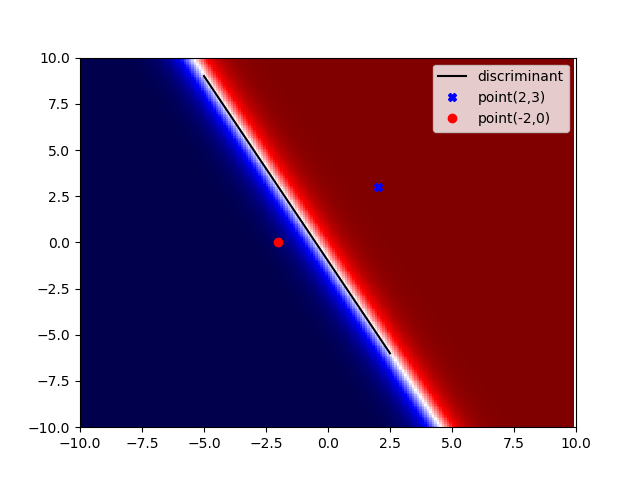
\includegraphics[scale=0.6]{ex1_a.png} 

\\ 

We can also compute the prediction of the model for the two datapoints: 

$$ 

\text{prediction}_1 = sign(w^\top x_1) = sign(8) = 1 \ne -1 

$$ 

$$ 

\text{prediction}_2 = sign(w^\top x_2) = sign(-3) = -1 \ne 1 

$$ 

So our two datapoints are missclassified, now we can say that on the plot below 

area in red (upper right of the plot) represents the area classified as class $1$ by our model and 

blue (lower left part of the plot) is for class $-1$ 



\subsection{Part b} 

After one iteration of a batch learning algorithm we get the following new discriminant: 

$$ 

w_{new} = w_{old} + \eta\sum_{i=1}^N x_ic_i 

$$ 

$$ 

w_{new} = \begin{bmatrix}-2.5 & -1.5 & -2.5\end{bmatrix} 

$$ 

And now, both data points are acorrectly classified by the new model: 

\\ 

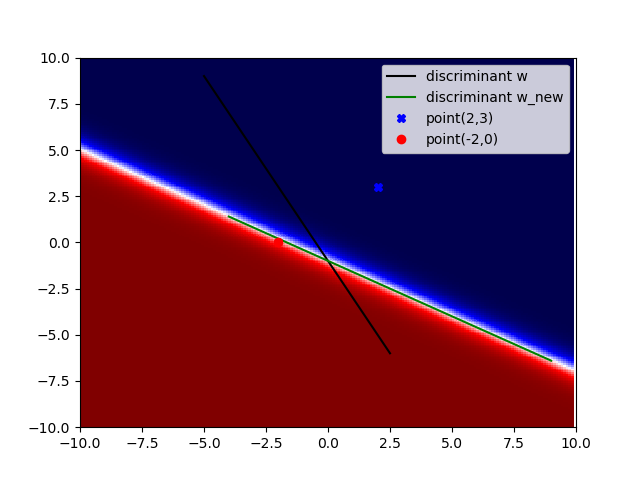
\includegraphics[scale=0.6]{ex1_b.png} 



\subsection{Part c} 

Learning is an iterative process. In a batch version learning, at each iteration we compute a new model 

based on the whole dataset whereas in a stochastic version, at each iteration we pick up a single data in the dataset 

and we base our computation on this data point only. 

\\ 

When the dataset becomes too big, the computation time of a batch iteration is going to need ressources 

proportional to the size of the dataset and a stochastic iteration will always use the same amount of ressources 

independantly of the size of the dataset. 



\subsection{Part d} 

When applying the stochastic algorithm, we get the following (different) result: 

$$ 

w_{new} = \begin{bmatrix}1 & -0.4 & -0.8\end{bmatrix} 

$$ 

And again, both points are correctly classified after the complete sweep: 

\\ 

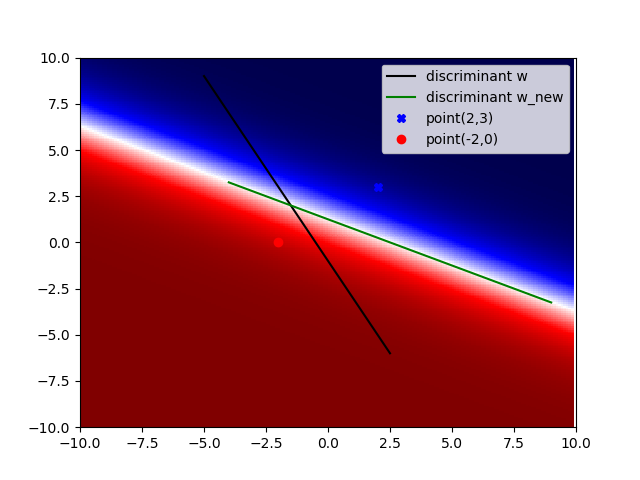
\includegraphics[scale=0.6]{ex1_d.png} 


\section{Exercise 2: Logistic classification \& discrimination}

\subsection{Part a}
Initialize $w_0$ ?
\begin{enumerate}
    \item Some fixed $w_0$ like $\begin{bmatrix}0 & 0 & \cdots & 1\end{bmatrix}$
    \item Some computation around the dataset like the mean: $w_0 = \frac{1}{N}\sum_{i=1}^N x_i$, concatenated with a constant.
    \item Some random vector
\end{enumerate}
How to learn: for batch learning use this equation at each step
$$
w_{n+1} = w_n - \eta \nabla E(w_n) = w_n - \eta \sum_{n=1}^{N}\left(y(n)-t_n\right)x_n
$$
How to stop the iterative process ?
\begin{enumerate}
\item Stop when the norm of the difference vector is low: $\Delta_n = \frac{\left\Vert w_{n+1} - w_n\right\Vert}{\left\Vert w_n \right\Vert} < \epsilon$
\\
This is a commonly used criterion that stops the process when the steps we take are getting small compared to our current result.
\item Stop after fixed number of iteration
\\
This ensures we won't enter in a infinite non-convergent process. 
\item Stop when a threshold error is reached: $E(w_n) < \epsilon $
\\
This is actually a bad idea because most of the time we can't be certain it is possible to reach such threshold on the error.
It would result in an infinite process.
\end{enumerate}
Our algorithm goes as follows:
\begin{enumerate}
    \item Chose $\epsilon$, $N$ and $\eta$ respectivelly for precision, maximum number of iterations and speed convergency.
    \item Set current error $\Delta$ to $+\infty$ and $n$ to $0$
    \item Chose the initial discriminant: $w_{current}$. WE NEED TO CHOSE THE METHOD ! 
    \item While $\Delta > \epsilon \wedge n < N$ do
    \begin{enumerate}
        \item Compute and store next discriminant $w_{next}$:
$$
w_{next} = w_{current} - \eta \sum_{n=1}^{N}\left(\sigma({w_{current}}^\top x_n)-t_n\right)x_n
$$
        \item Compute and store the new error $\Delta$:
$$
\Delta = \frac{\left\Vert w_{next} - w_{current}\right\Vert}{\left\Vert w_{current} \right\Vert}
$$
        \item Prepare for next iteration: store $w_{next}$ in place of $w_{current}$ and increment $n$
    \end{enumerate}
    \item If $\Delta > \epsilon$, it means we have not converged enough towards the limit. We should consider increasing N OR using another algorithm for convergence (eg. Newton-Raphson)
    \item Result is stored in $w_{current}$, number of steps in $n$. 
\end{enumerate}


\end{document}

\begin{lstlisting}
    # Some python code
\end{lstlisting}